\documentclass[11pt, oneside]{article}   	% use "amsart" instead of "article" for AMSLaTeX format
\usepackage{geometry}                		% See geometry.pdf to learn the layout options. There are lots.
\geometry{letterpaper}                   		% ... or a4paper or a5paper or ... 
%\geometry{landscape}                		% Activate for rotated page geometry
%\usepackage[parfill]{parskip}    		% Activate to begin paragraphs with an empty line rather than an indent
\usepackage{graphicx}				% Use pdf, png, jpg, or eps§ with pdflatex; use eps in DVI mode
								% TeX will automatically convert eps --> pdf in pdflatex
\usepackage{amssymb}
\usepackage{amsmath}
\usepackage{algorithm}% http://ctan.org/pkg/algorithm
\usepackage{algpseudocode}% http://ctan.org/pkg/algorithmicx
\usepackage{mathtools,xparse}
%SetFonts

%SetFonts


\title{CSE512 HW3}
\author{Tim Zhang (110746199)}
\date{}							% Activate to display a given date or no date

\begin{document}
\maketitle
%\section{}
%\subsection{}

\DeclarePairedDelimiter{\norm}{\lVert}{\rVert}

\section{Support Vector Machines}
\subsection{Question 1: Primal and Dual of Kernel SVM}
\subsubsection{Part A}
Using the observation that maximizing $\alpha$ is the same as minimizing $-\alpha$ we can rewrite the dual objective as follows:
\begin{gather*}
\min_{\alpha} \frac{1}{2} \sum_{i = 1}^m\sum_{j = 1}^m \alpha_i \alpha_j y_i y_j k(\boldsymbol{x}_i , \boldsymbol{x}_j) - \sum_{j = 1}^m \alpha_j
\end{gather*}
Which gives the following quadprog parameters with the custom matrix K being specified in words and implemented specifically for each kernel function.
\begin{verbatim}
% K is the mxm matrix of the kernel function applied as k(x_i, x_j)
% So H is composed of y_i * y_j * k(x_i, x_j)
H = (y * y') .* K;
f = -1 * ones(m, 1);

% There are no constraints
A = [];
b = [];
Aeq = [];
beq = [];

% Using bounds on alpha to handle inequality constraints
lb = zeros(m, 1);
ub = C * ones(m, 1);
\end{verbatim}

\newpage{}
\subsubsection{Part B}
Rewriting $(1)$ in the equivalent constrained formulation we have:
\begin{gather*}
\min_{\boldsymbol{w} \in \mathbb{R}^d, \text{ } \xi \in \mathbb{R}^m} \frac{1}{2} \norm{\boldsymbol{w}}_2^2 + C\sum_{i = 1}^m \xi_i\\
\text{s.t. } -(y_i \langle \boldsymbol{w}, \phi(\boldsymbol{x}_i) \rangle - 1 + \xi_i) \leq 0\\
-\xi_i \leq 0
\end{gather*}
The Lagrangian of the above constrained formulation using Lagrange multipliers $\alpha$ and $\gamma$:
\begin{gather*}
\frac{1}{2} \norm{\boldsymbol{w}}_2^2 + C\sum_{i = 1}^m \xi_i - \sum_{i = 1}^m \alpha_i(y_i \langle \boldsymbol{w}, \phi(\boldsymbol{x}_i) \rangle - 1 + \xi_i) - \sum_{i = 1}^m \gamma_i \xi_i
\end{gather*}
Computing the gradient with respect to $\boldsymbol{w}$:
\begin{gather*}
\nabla_w \frac{1}{2} \norm{\boldsymbol{w}}_2^2 + C\sum_{i = 1}^m \xi_i - \sum_{i = 1}^m \alpha_i(y_i \langle \boldsymbol{w}, \phi(\boldsymbol{x}_i) \rangle - 1 + \xi_i) - \sum_{i = 1}^m \gamma_i \xi_i\\
= \boldsymbol{w} - \sum_{i = 1}^m \alpha_i y_i \phi(\boldsymbol{x}_i)
\end{gather*}
Minimizing the Lagrangian with respect to $\boldsymbol{w}$:
\begin{gather*}
\boldsymbol{w} - \sum_{i = 1}^m \alpha_i y_i \phi(\boldsymbol{x}_i) = 0\\
\boldsymbol{w} = \sum_{i = 1}^m \alpha_i y_i \phi(\boldsymbol{x}_i) \text{ } \blacksquare
\end{gather*}

\newpage{}
\subsection{Question 2: Implement a kernel SVM using Quadratic Programming}
\subsubsection{Part A}
\begin{verbatim}
%
% Trains on kernel SVM dual objective.
%
function alpha = train_ksvm_dual(X, y, C, kernel, gamma)
    [m, d] = size(X);
    
    % K is the mxm matrix of the kernel function applied as k(x_i, x_j)
    if strcmp('gaussian', kernel)
        K = zeros(m, m);
        
        % Compute K(x_i, x_j) for each i, j
        for i = 1:m
            for j = 1:m
                K(i, j) = exp((-1 * gamma) * norm(X(i, :) - X(j, :))^2);
            end
        end
    elseif strcmp('linear', kernel)
        K = X * X';
    end
    
    % So H is composed of y_i * y_j * k(x_i, x_j)
    H = (y * y') .* K;
    f = -1 * ones(m, 1);
    
    % There are no constraints
    A = [];
    b = [];
    Aeq = [];
    beq = [];
    
    % Using bounds on alpha to handle inequality constraints
    lb = zeros(m, 1);
    ub = C * ones(m, 1);
    
    [alpha, value] = quadprog(H, f, A, b, Aeq, beq, lb, ub);
    
    disp('Objective value: '); disp(value);
end
\end{verbatim}

\subsubsection{Part B}
\begin{verbatim}
%
% Main.
% All input is expected to be mxd dimensional
% Ex: driver(Xtr', ytr', Xte', yte', 10, 'linear', .001)
%
function driver(Xtr, ytr, Xte, yte, C, kernel, gamma)
    alpha = train_ksvm_dual(Xtr, ytr, C, kernel, gamma);
    ypredicted = test_ksvm_dual(alpha, Xtr, ytr, Xte, kernel, gamma);
    
    % Calculate prediction accuracy
    [m, d] = size(yte);
    misclassified = 0;
    
    for i = 1: m
        if yte(i) ~= ypredicted(i)
            misclassified = misclassified + 1;
        end
    end
    
    accuracy = double(length(yte) - misclassified)/length(yte);
    
    disp('Accuracy: '); disp(accuracy);
    
    % Count support vectors
    supports = 0;
    [alpha_m, alpha_d] = size(alpha);
    
    for i = 1: alpha_m
        if alpha(i) > C/100
            supports = supports + 1;
        end
    end
    
    disp('Support Vectors: '); disp(supports);
end

%
% Generates predicted y via learned w for each x.
%
function ypredicted = test_ksvm_dual(alpha, Xtr, ytr, Xte, kernel, gamma)
    [m, d] = size(Xtr);      % Dimensions of train
    w = zeros(1, d);         % Weight vector
    [mte, dte] = size(Xte);  % Dimensions of test
    ypredicted = 1:mte;      % Output vector
    
    % Compute w
    if strcmp('gaussian', kernel)
        % For each test sample
        for i = 1: mte
            % Compute the predicted value of the test
            prediction = 0;
            
            for j = 1: m
                prediction = prediction + 
                (alpha(j) * ytr(j) * exp((-1 * gamma) * norm(Xtr(j, :) - Xte(i, :))^2));
            end
            
            if prediction > 0
                ypredicted(i) = 1;
            else
                ypredicted(i) = -1;
            end
        end
        
    elseif strcmp('linear', kernel)
        % Use formulation from Q1
        for i = 1: m
            w = w + (alpha(i) * ytr(i) * Xtr(i, :));
        end
        
        for i = 1: mte
            if Xte(i, :) * w' > 0
                ypredicted(i) = 1;
            else
                ypredicted(i) = -1;
            end
        end
    end
end
\end{verbatim}

\subsubsection{Part C}
To discriminate which $\alpha_i$ corresponded to a support vector the value of $\alpha_i$ was compared against $C/100$.
\begin{verbatim}
Linear Kernel, C = 10
    Accuracy: 0.8446
    Support Vectors: 1803
    Value: -1.7544e+04

Gaussian Kernel, C = 10
    Accuracy: 0.8516
    Support Vectors: 2078
    Value: -1.9467e+04
\end{verbatim}

\subsubsection{Part D}
\begin{verbatim}
Linear Kernel, C = .1
    Accuracy: 0.8476
    Support Vectors: 1926
    Value: -183.2313
    
Gaussian Kernel, C = .1
    Accuracy: 0.7596
    Support Vectors: 2961
    Value: -251.3329
\end{verbatim}

\newpage{}
\subsection{Question 3: Implement Linear SVM using Sub-Gradient Descent}
\subsubsection{Part A}
Computing the subgradient of $L(\boldsymbol{w})$:
\begin{gather*}
\partial_w \frac{1}{2} \norm{\boldsymbol{w}}_2^2 + C \sum_{j = 1}^m \ell(\boldsymbol{w}, \phi(\boldsymbol{x}_j)
, y_j)\\
= \boldsymbol{w} + C \sum_{j = 1}^m \begin{cases} 0, & \mbox{if } 1 - y_j \langle \boldsymbol{w}, \phi(\boldsymbol{x}_j) \rangle < 0 \\ -y_j \phi(\boldsymbol{x}_j), & \mbox{if } 1 - y_j \langle \boldsymbol{w}, \phi(\boldsymbol{x}_j) \rangle \geq 0 \end{cases}\\
= \boldsymbol{w} - C \sum_{(\boldsymbol{x}, y): 1 - y_j \langle \boldsymbol{w}, \phi(\boldsymbol{x}_j) \rangle \geq 0} y \phi(\boldsymbol{x}_j)
\end{gather*}
Which yields the Sub-Gradient Descent update rule:
\begin{gather*}
\boldsymbol{w}_{t + 1} \leftarrow \boldsymbol{w}_t - \eta_t \partial_w L(\boldsymbol{w}_t)\\
\equiv \boldsymbol{w}_{t + 1} \leftarrow \boldsymbol{w}_t - \eta_t (\boldsymbol{w}_t - C \sum_{(\boldsymbol{x}, y): 1 - y_j \langle \boldsymbol{w}, \phi(\boldsymbol{x}) \rangle \geq 0} y \phi(\boldsymbol{x}))\\
\equiv \boldsymbol{w}_{t + 1} \leftarrow \boldsymbol{w}_t - \eta_t  \boldsymbol{w}_t + \eta_t C \sum_{(\boldsymbol{x}, y): 1 - y_j \langle \boldsymbol{w}, \phi(\boldsymbol{x}) \rangle \geq 0} y \phi(\boldsymbol{x})\\
\equiv \boldsymbol{w}_{t + 1} \leftarrow (1 - \eta_t) \boldsymbol{w}_t + \eta_t C \sum_{(\boldsymbol{x}, y): 1 - y_j \langle \boldsymbol{w}, \phi(\boldsymbol{x}) \rangle \geq 0} y \phi(\boldsymbol{x}) \text{ } \blacksquare
\end{gather*}

\newpage{}
\subsubsection{Part B}
\begin{verbatim}
%
% Trains linear SVM using subgradient descent
% All input is expected to be mxd dimensional
% Ex: train_svm_sgd(Xtr', ytr', 10, 1, 100)
%
function [w] = train_svm_sgd(X, y, C, a, T)
    [m, d] = size(X);   % Dimensions of data
    w_t = zeros(d, 1);  % Initialize w_0 = 0
    w = w_t;            % dx(T + 1) matrix of w_t from each iteration including w_0
    
    % Run algorithm T iterations
    for t = 1: T
        eta = a/t;  % Weight decay
        sum = 0;    % Misclassified sum
        
        % Calculate summation of misclassified
        for i = 1: m
            if y(i) * (X(i, :) * w_t) <= 1
                sum = sum + y(i) * X(i, :)';
            end
        end
        
        w_t = ((1 - eta) * w_t) + (eta * C * sum);
        
        w = [w w_t];  % Return each w_t in w
    end
end
\end{verbatim}

\newpage{}
\subsubsection{Part C}
The algorithm was run as $\verb![w_10] = train_svm_sgd(Xtr', ytr', 10, 1, 10000)!$ and $\verb![w_01] = train_svm_sgd(Xtr', ytr', .01, 1, 10000)!$ for the following sections.  

The weight matrices were then passed into $\verb!plot(w, Xte, yte, Xtr, ytr, C)!$ given below.  

NOTE: I printed each figure individually and commented out the other figures when I was not considering them, this may cause the code not to run as is or only print a single graph at a time instead of all three.

\begin{verbatim}
%
% Calculates various observations from data
%
function plot(w, Xte, yte, Xtr, ytr, C)
    [~, T] = size(w);
    train = calculateError(w, Xtr, ytr);
    test = calculateError(w, Xte, yte);
    objective = calculateObjective(w, Xtr, ytr, C);
    
    % Plot objective function    
    figure,
    loglog(objective');
    
    % Plot training error
    figure,
    plot(1:T, train);

    % Plot test error
    figure,
    plot(1:T, test);
end











%
% Calculates objective value
%
function value = calculateObjective(w, X, y, C)
    [~, T] = size(w);     % Dimensions of weights
    [m, d] = size(X);     % Dimensions of X
    value = zeros(T, 1);  % Value for each iteration
    
    % Calculate objective value for each w_t
    for t = 1: T
        sum = 0;
        
        % Calculate summation term
        for i = 1: m
            sum = sum + max(0, 1 - (y(i) * (X(i, :) * w(:, T))));
        end
        value(t) = (.5 * norm(w(:, t))^2) + (C * sum);
    end    
end

%
% Calculates empirical error
%
function error = calculateError(w, X, y)
    [~, T] = size(w);     % Dimensions of weights
    [m, d] = size(X);     % Dimensions of X
    error = zeros(T, 1);  % Error for each iteration
    
    % Calculate empirical error for each w_t
    for t = 1: T
        loss = 0;
        
        for i = 1: m
            if y(i) * (X(i, :) * w(:, t)) < 0
                loss = loss + 1;
            end
        end
        error(t) = loss/m;
    end
end
\end{verbatim}

\newpage{}
\subsubsection{Part D}
\begin{figure}[h!]
  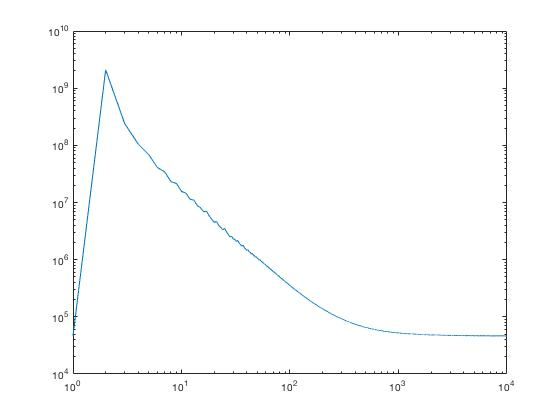
\includegraphics[width=\linewidth]{objective_10.jpg}
  \caption{Log-log objective values for C = 10}
\end{figure}

\newpage{}
\begin{figure}[h!]
  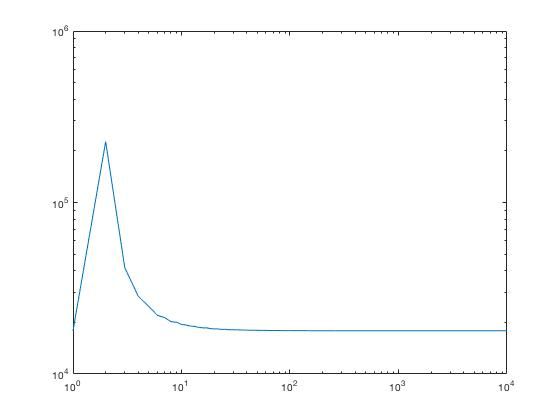
\includegraphics[width=\linewidth]{objective_01.jpg}
  \caption{Log-log objective values for C = .1}
\end{figure}
In both cases of C it seems as though the algorithm converges to the roughly similar values.  However when C = .1 the algorithm converges much faster and more dramatically than when C = 10.

\newpage{}
\subsubsection{Part E}
\begin{figure}[h!]
  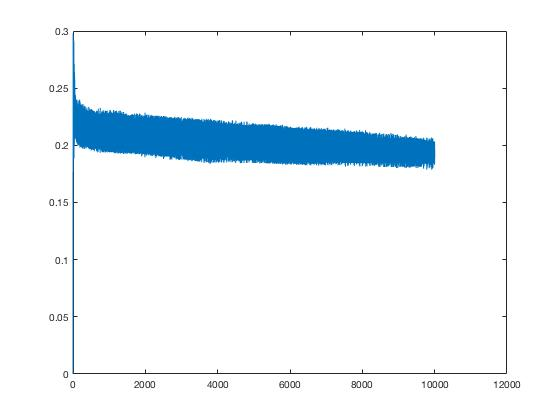
\includegraphics[width=\linewidth]{training_loss_10.jpg}
  \caption{Training error for C = 10}
\end{figure}
At the best point in the search the training error is around $.17$ which is a little worse than the $\verb!quadprog!$ formulation for test error at C = 10.

\newpage{}
\begin{figure}[h!]
  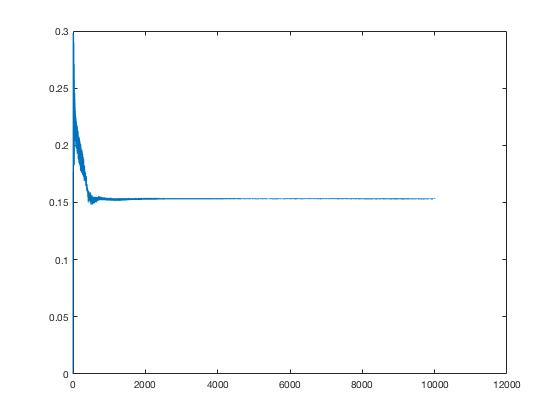
\includegraphics[width=\linewidth]{training_loss_01.jpg}
  \caption{Training error for C = .1}
\end{figure}
At the best point in the search the training error is around $.145$ which is roughly as good as the $\verb!quadprog!$ formulation for test error at C = .1

\newpage{}
\subsubsection{Part F}
\begin{figure}[h!]
  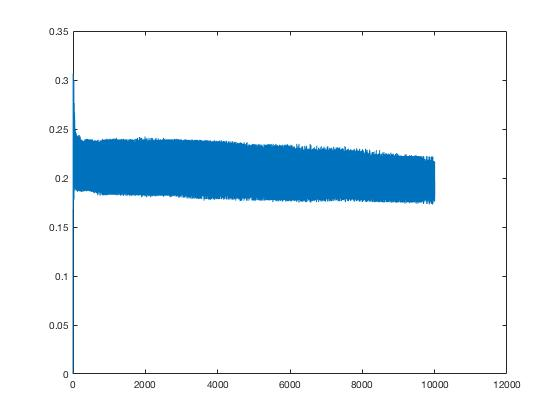
\includegraphics[width=\linewidth]{test_error_10.jpg}
  \caption{Test error for C = 10}
\end{figure}
The test error is best around .17, which is comparable to the test error using $\verb!quadprog!$.
\newpage{}
\begin{figure}[h!]
  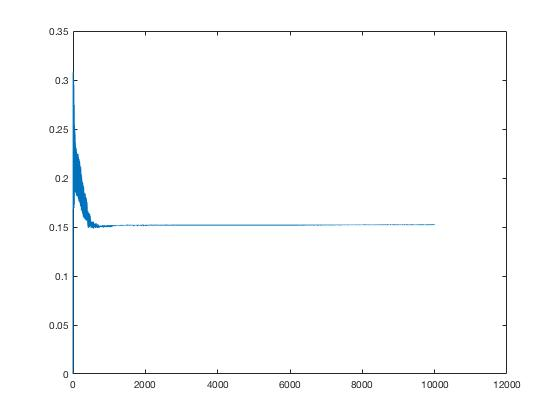
\includegraphics[width=\linewidth]{test_error_01.jpg}
  \caption{Test error for C = .1}
\end{figure}
The test error achieves the best loss at around .15 which is an 85\% accuracy rate which is slightly better than the $\verb!quadprog!$ implementation.
\newpage{}
\subsection{Question 4: Invariance to Additive Constants in Kernels}
Adding a constant $c$ to the kernel function yields the following dual formulation:
\begin{gather*}
\max_{\alpha} \sum_{j = 1}^m \alpha_j - \frac{1}{2} \sum_{i = 1}^{m}\sum_{j = 1}^{m} y_i\alpha_i y_j \alpha_j (k(\boldsymbol{x}_i , \boldsymbol{x}_j) + c)\\
= \max_{\alpha} \sum_{j = 1}^m \alpha_j - \frac{1}{2} \Big( \sum_{i = 1}^{m}\sum_{j = 1}^{m} y_i\alpha_i y_j \alpha_j k(\boldsymbol{x}_i , \boldsymbol{x}_j) + c \sum_{i = 1}^{m}\sum_{j = 1}^{m} y_i\alpha_i y_j \alpha_j \Big)\\
= \max_{\alpha} \sum_{j = 1}^m \alpha_j - \frac{1}{2} \Big( \sum_{i = 1}^{m}\sum_{j = 1}^{m} y_i\alpha_i y_j \alpha_j k(\boldsymbol{x}_i , \boldsymbol{x}_j) + c \Big( \sum_{i = 1}^{m} y_i\alpha_i \Big) \Big( \sum_{j = 1}^{m} y_j \alpha_j \Big) \Big)\\
= \max_{\alpha} \sum_{j = 1}^m \alpha_j - \frac{1}{2} \Big( \sum_{i = 1}^{m}\sum_{j = 1}^{m} y_i\alpha_i y_j \alpha_j k(\boldsymbol{x}_i , \boldsymbol{x}_j) + 0 \Big)\\
= \max_{\alpha} \sum_{j = 1}^m \alpha_j - \frac{1}{2} \sum_{i = 1}^{m}\sum_{j = 1}^{m} y_i\alpha_i y_j \alpha_j k(\boldsymbol{x}_i , \boldsymbol{x}_j)\\
\text{s.t.} \sum_j^m y_j \alpha_j = 0\\
0 \leq \alpha_j \leq C \text{ } \forall j
\end{gather*}

Where the constraints are applied at each step of the derivation and the final formula is the normal dual formulation using $k(\boldsymbol{x}_i, \boldsymbol{x}_j)$ $\blacksquare$

\newpage{}
\section{Kernel Ridge Regression}
\subsection{Question 5: Alternative Formulation for the Solution of Ridge Regression}
\subsubsection{Part A}
Using equation (8) and taking $\alpha = \boldsymbol{y} - X\boldsymbol{w}_\lambda$ we find:
\begin{gather*}
m\lambda \boldsymbol{w}_\lambda = X^\top (\boldsymbol{y} - X\boldsymbol{w}_\lambda)\\
\equiv Xm\lambda \boldsymbol{w}_\lambda = XX^\top \alpha\\
\equiv X\boldsymbol{w}_\lambda = \frac{1}{m\lambda}XX^\top \alpha\\
\equiv -\alpha + \boldsymbol{y}= \frac{1}{m\lambda}XX^\top \alpha\\
\equiv \boldsymbol{y}= \frac{1}{m\lambda}XX^\top \alpha + \alpha\\
\equiv \frac{1}{m\lambda}XX^\top \alpha + \alpha = \boldsymbol{y} \text{ } \blacksquare
\end{gather*}

\subsubsection{Part B}
Solving for $\alpha$:
\begin{gather*}
\frac{1}{m\lambda}XX^\top \alpha + \alpha = \boldsymbol{y}\\
\equiv (\frac{1}{m\lambda}XX^\top + I_m) \alpha = \boldsymbol{y}\\
\equiv \alpha = (\frac{1}{m\lambda}XX^\top + I_m)^{-1} \boldsymbol{y} \text{ } \blacksquare
\end{gather*}

\subsubsection{Part C}
Solving for $\boldsymbol{w}_\lambda$:
\begin{gather*}
m\lambda \boldsymbol{w}_\lambda = X^\top \alpha\\
\equiv m\lambda \boldsymbol{w}_\lambda = X^\top (\frac{1}{m\lambda}XX^\top + I_m)^{-1} \boldsymbol{y}\\
\equiv \boldsymbol{w}_\lambda = X^\top \frac{1}{m\lambda} (\frac{1}{m\lambda}XX^\top + I_m)^{-1} \boldsymbol{y}\\
\equiv \boldsymbol{w}_\lambda = X^\top (m\lambda(\frac{1}{m\lambda}XX^\top + I_m))^{-1} \boldsymbol{y}\\
\equiv \boldsymbol{w}_\lambda = X^\top (XX^\top + m\lambda I_m)^{-1} \boldsymbol{y} \text{ } \blacksquare
\end{gather*}

\newpage{}
\subsection{Question 6: Implement Kernel Ridge Regression}
\subsubsection{Part A}
\begin{verbatim}
%
% Calculates alpha using the solution of 5b
%
function alpha = train_krr(X, y, lambda, kernel, gamma)
    [m, ~] = size(X);  % Dimensions of data
    kX = zeros(m, m);  % Holds the value of the kernel
    
    if strcmp('gaussian', kernel)
        % Construct each element of XX^T via kernel function application
        for i = 1: m
            for j = 1: m
                kX(i, j) = exp((-1 * gamma) * norm(X(i,:) - X(j, :))^2);
            end
        end
        
        alpha = inv((1/(m * lambda)) * kX + eye(m)) * y;
        
    elseif strcmp('linear', kernel)
        % Directly compute alpha
        alpha = inv((1/(m * lambda)) * (X * X') + eye(m)) * y;
    end   
end
\end{verbatim}

\newpage{}
\subsubsection{Part B}
Using $\boldsymbol{w}_\lambda = \frac{1}{m\lambda }X^\top \alpha$.
\begin{verbatim}
%
% Implementation of Kernel Ridge Regression
%
function kernelRidgeRegression(Xtr, ytr, Xte, yte, lambda, kernel, gamma)
    alpha = train_krr(Xtr, ytr, lambda, kernel, gamma);
    ypredicted = test_krr(alpha, Xtr, ytr, Xte, lambda, kernel, gamma);
    
    % Calculate prediction accuracy
    [m, ~] = size(yte);
    misclassified = 0;
    
    for i = 1: m
        if yte(i) ~= ypredicted(i)
            misclassified = misclassified + 1;
        end
    end
    
    accuracy = double(length(yte) - misclassified)/length(yte);
    
    disp('Test Accuracy: ');
    disp(accuracy);
end
\end{verbatim}

\newpage{}
\begin{verbatim}
%
% Computes predicted values of test samples
%
function ypredicted = test_krr(alpha, Xtr, ytr, Xte, lambda, kernel, gamma)
    [m, d] = size(Xtr);    % Dimensions of training data
    [mte, ~] = size(Xte);  % Dimensions of test data
    w = d:1;               % Weight vector
    ypredicted = mte:1;    % Prediction vector
    
    if strcmp('gaussian', kernel)
        % Compute predictions
        for i = 1: mte
            
            ker = zeros(1, m);
            
            for j = 1: m
                ker(j) = exp((-1 * gamma) * norm(Xtr(j,:) - Xte(i, :))^2);
            end
            
            if (1/(m * lambda)) * ker * alpha > 0
                ypredicted(i) = 1;
            else
                ypredicted(i) = -1;
            end
        end
        
        % Compute training error
        misclassified = 0;

        for i = 1: m
            ker = zeros(1, m);
            
            for j = 1: m
                ker(j) = exp((-1 * gamma) * norm(Xtr(j,:) - Xtr(i, :))^2);
            end
            
            if ytr(i) * (1/(m * lambda)) * ker * alpha < 0
                misclassified = misclassified + 1;
            end
        end
        
    elseif strcmp('linear', kernel)
        w = (1/(m * lambda)) * Xtr' * alpha;
        
        % Compute predictions
        for i = 1: mte
            if Xte(i, :) * w > 0
                ypredicted(i) = 1;
            else
                ypredicted(i) = -1;
            end
        end
        
        % Compute training error
        misclassified = 0;

        for i = 1: m
            if ytr(i) * Xtr(i, :) * w < 0
                misclassified = misclassified + 1;
            end
        end
    end

    % Output accuracy
    accuracy = double(m - misclassified)/m;
    disp('Training Accuracy: ');
    disp(accuracy); 
end
\end{verbatim}

\newpage{}
\subsubsection{Part C}
$\verb!Linear Kernel, ! \lambda \verb! = .00002!$\\
$\verb!    Test Accuracy: 0.8461!$\\
$\verb!    Training Accuracy: 0.8448!$\\\\
$\verb!Gaussian Kernel, ! \lambda \verb! = .00002!$\\
$\verb!    Test Accuracy: 0.8521!$\\
$\verb!    Training Accuracy: 0.8402!$


\subsubsection{Part D}
$\verb!Linear Kernel, ! \lambda \verb! = .002!$\\
$\verb!    Test Accuracy: 0.8486!$\\
$\verb!    Training Accuracy: 0.8420!$\\\\
$\verb!Gaussian, ! \lambda \verb! = .002!$\\
$\verb!    Test Accuracy: 0.7616!$\\
$\verb!    Training Accuracy: 0.7476!$
\end{document} 